\section{Podzadanie A}
\subsection{Rozkład danych}
Celem podzadania A było wyznaczenie trafności odpowiedzi na pytanie. Z dostarczonego zbioru danych udało się uzyskać ~30 000 przykładów uczących w postaci par pytanie-odpowiedź o różnych etykietach wyrażających trafność odpowiedzi na zadane pytanie. 
Aby uzyskać pewność, że model będzie sobie radził z nowymi danymi wykorzystano metodę statystyczną zwaną sprawdzianem krzyżowym. Zbiór danych został losowo podzielony na zbiór uczący i walidujący w proporcji 4:1. Pozwoliło to uzyskać ~24000 przypadków uczących i ~6000 przypadków walidujących. Po połączeniu klas ,,PotentiallyUseful'' i ,,Bad'' w jedną klasę ,,Bad'' rozkład etykiet w obu zbiorach był następujący:

\begin{table}[H]
\caption{Rozkład klas w zbiorze uczącym}
\label{train_set_statistics_score_table}
    \begin{center}
        \begin{tabular}{ |c|c| } 
            \hline
            klasa & rozkład\\
            \hline
            ,,Good'' & 36,951\% \\
            \hline
            ,,Bad'' & 63,049\% \\
            \hline
        \end{tabular}
    \end{center}
\end{table}

\begin{table}[H]
\caption{Rozkład klas z zbiorze walidującym}
\label{train_set_statistics_score_table}
    \begin{center}
        \begin{tabular}{ |c|c| } 
            \hline
            klasa & rozkład\\
            \hline
            ,,Good'' & 36,277\% \\
            \hline
            ,,Bad'' & 63,723\% \\
            \hline
        \end{tabular}
    \end{center}
\end{table}
\subsection{Miary statystyczne}
W celu rozwiązania problemu klasyfikacji podjęto próby wykorzystania wcześniej zdefiniowanych miar statystycznych. Pierwszą próbą było sprawdzenie zależności między wartością bezwzględną różnicy długości odpowiedzi i pytania, a stopniem trafności odpowiedzi na pytanie (rysunek~\ref{fig:mstatystyczna}).


\begin{figure}[H]
\caption{Zależność różnicy długości i klasy. \label{fig:mstatystyczna}}
\centering
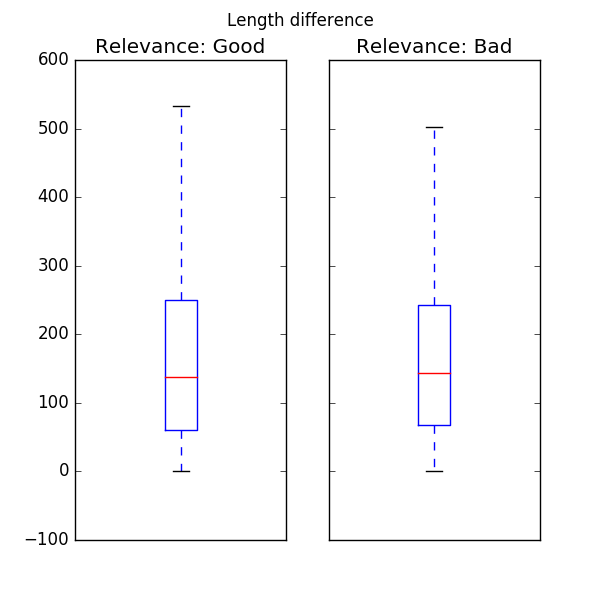
\includegraphics[scale=0.5]{subtask_a_length_difference.png}
\end{figure}

Wartości mediany, pierwszego kwartylu, trzeciego kwartylu są do siebie bardzo zbliżone dla obu wykresów. Również wartości minimalne i maksymalne wykazują podobne wartości. Widać że nie ma większej zależności pomiędzy różnicą długości tekstów, a ich klasą trafności. 
Następną sprawdzoną metryką była zależność pomiędzy indeksem Jaccarda, a trafnością odpowiedzi (rysunek~\ref{fig:jaccarda}). 



\begin{figure}[H]
\caption{Zależność odległości Jaccarda i klasy. \label{fig:jaccarda}}
\centering
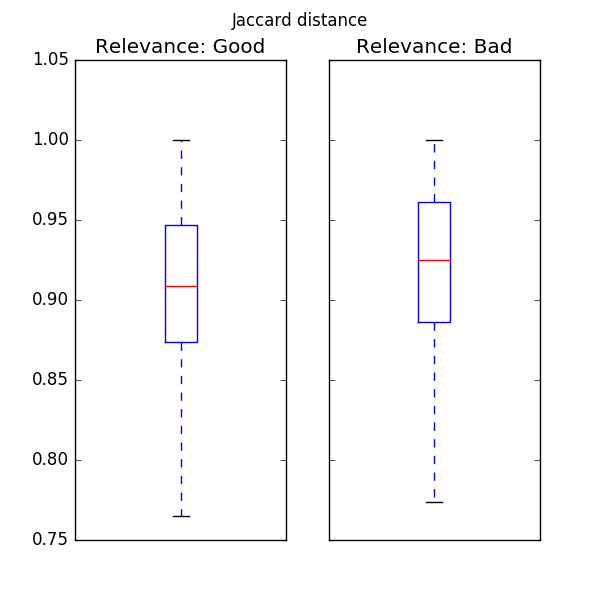
\includegraphics[scale=0.5]{subtask_a_jaccard_distance.png}
\end{figure}

Odnotowano nieznaczne różnice pomiędzy wartościami kwartylu dla obu klas trafności. Różnice pokrywają się z naturą odległości Jaccarda która powinna być większa dla mniej podobnych zbiorów. Widać, że dla klasy ,,BAD'' wartości kwartyli są większe.
  
Ostatnią wykorzystaną metryką była zależność pomiędzy odległością cosinusową, a trafnością odpowiedzi (rysunek~\ref{fig:trafsnosca}). 



\begin{figure}[H]
\caption{Zależność podobieństwa kosinusowego i klasy. \label{fig:trafsnosca}}
\centering
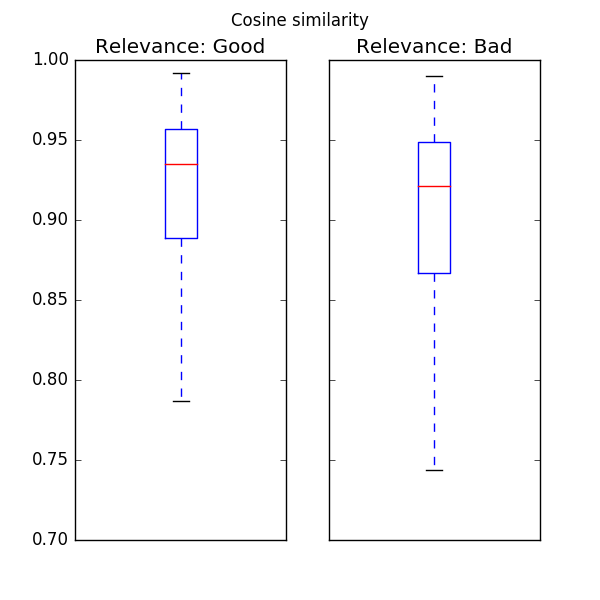
\includegraphics[scale=0.5]{subtask_a_cosine_similarity.png}
\end{figure}

W tym przypadku również wykazano nieznaczne różnice pomiędzy wartościami kwartylu dla obu klas trafności. Różnice pokrywają się z naturą podobieństwa cosinusowego które powinno być większa dla bardziej podobnych zbiorów. Widać że dla klasy ,,GOOD'' wartości kwartyli są większe. 

Na podstawie opracowanych miar statystycznych stworzono klasyfikator oparty na regresji logistycznej (tablice~\ref{tab:train_set_statistics_score_table} i \ref{tab:train_set_statistics_score_table}). Niestety skuteczność tego rozwiązania nie była zadowalająca.

\begin{table}[H]
\caption{Skuteczność regresji logistycznej na zbiorze uczącym. \label{tab:train_set_statistics_score_table}}
    \begin{center}
        \begin{tabular}{ |c|c| } 
            \hline
            metryka & wartość\\
            \hline
            Accuracy & 0,633 \\
            \hline
            Precission & 0,660 \\
            \hline
            Recall & 0,009 \\ 
            \hline
        \end{tabular}
    \end{center}
\end{table}

\begin{table}[H]
\caption{Skuteczność regresji logistycznej na zbiorze walidującym. \label{tab:train_set_statistics_score_table}}
    \begin{center}
        \begin{tabular}{ |c|c| } 
            \hline
            metryka & wartość\\
            \hline
            Accuracy & 0,626 \\
            \hline
            Precission & 0,760 \\
            \hline
            Recall & 0,010 \\ 
            \hline
        \end{tabular}
    \end{center}
\end{table}



\subsection{Prosta sieć feed-forward}

W wyniku małej skuteczności rozwiązań opartych na statystyce podjęto pracę nad bardziej skomplikowanymi modelami - sieciami neuronowymi. Wypróbowano podstawową architekturę jaką jest sieć feed-forward. Składała się ona z jednej w pełni połączonej warstwy ukrytej o rozmiarze 64 jednostek. Na potrzeby wykorzystania sieci neuronowej potrzebna była reprezentacja zdania w formie wektorowej. Każde zdanie zostało zamienione w wektor według wzoru:

%\[
\begin{equation}
\overrightarrow{V} = \frac{\sum_{i=1}^{n}\overrightarrow{s_i}}{n}
\end{equation}
%\]
Gdzie:
\begin{itemize}
\item $n$ - liczba słów w zdaniu,
\item $s$ - word-embedding dla $i$-tego słowa,
\item $V$ - wektorowa reprezentacja zdania.
\end{itemize}

Wejściem sieci były dwa wektory (pytanie i komentarz) połączone w jeden. Wyjściem sieci był pojedynczy neuron wyrażający wyliczoną przez sieć trafność pytania dla odpowiedzi (zob. rysunek~\ref{fig:ffa}).


\begin{figure}[H]
\caption{Architektura sieci. \label{fig:ffa}}
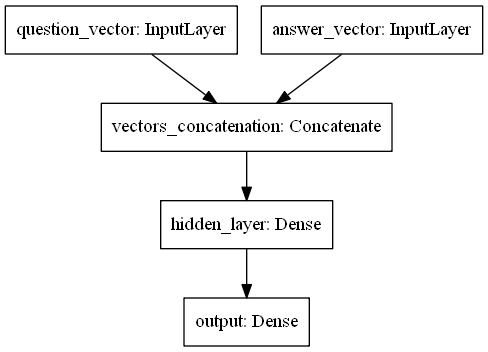
\includegraphics[scale=0.4]{subtask_a_feedforward_model}
\centering
\end{figure}

Sieć zostałą przeuczona zbiorem trenującym, a następnie jej skutecznośc została sprawdzona zbiorem walidującym. Poniżej wykres przedstawiający przebieg uczenia dla 400 epok (rysunki~\ref{fig:ffloss} i \ref{fig:ffacc}).

\begin{figure}[H]
\caption{Przebieg uczenia dla 400 epok (strata). \label{fig:ffloss}}
\centering
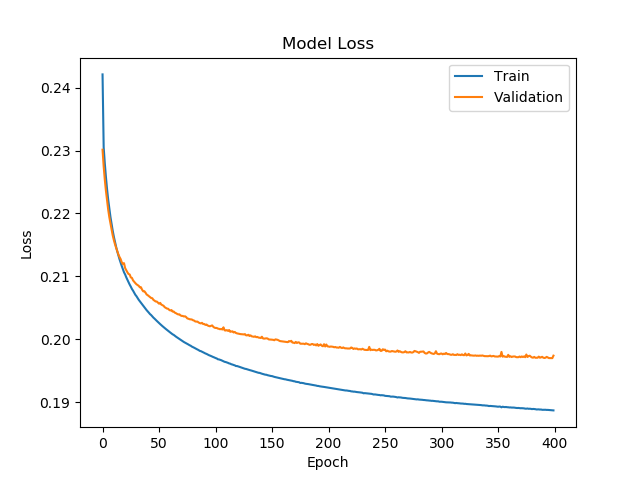
\includegraphics[scale=0.7]{subtask_a_feedforward_loss.png}
\end{figure}


\begin{figure}[H]
\caption{Przebieg uczenia dla 400 epok (trafność). \label{fig:ffacc}}
\centering
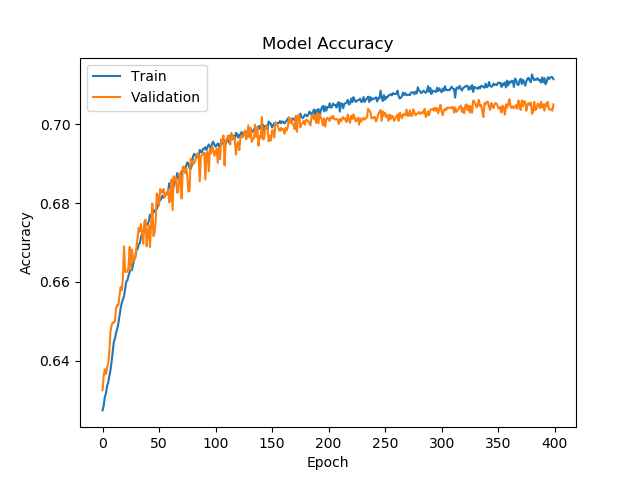
\includegraphics[scale=0.7]{subtask_a_feedforward_acc.png}
\end{figure}




\begin{table}[H]
\caption{Skuteczność sieci feedforward na zbiorze uczącym.\label{tab:ffu}}
\label{train_set_statistics_score_table}
    \begin{center}
        \begin{tabular}{ |c|c| } 
            \hline
            metryka & wartość\\
            \hline
            Accuracy & 0,716 \\
            \hline
            Precision & 0,667 \\
            \hline
            Recall & 0,460 \\ 
            \hline
        \end{tabular}
    \end{center}
\end{table}

\begin{table}[H]
\caption{Skuteczność sieci feedforward na zbiorze walidującym.\label{tab:ffw}}
\label{train_set_statistics_score_table}
    \begin{center}
        \begin{tabular}{ |c|c| } 
            \hline
            metryka & wartość\\
            \hline
            Accuracy & 0,705 \\
            \hline
            Precision & 0,449 \\
            \hline
            Recall & 0,633 \\ 
            \hline
        \end{tabular}
    \end{center}
\end{table}


Rozwiązanie okazało się skuteczne, udało się zwiększyć trafność klasyfikacji o kilka procent (tablice~\ref{tab:ffu} i \ref{tab:ffw}). 


\subsection{Sieć syjamska}

Ostatnią realizowaną architekturą była dużo bardziej skomplikowana sieć syjamska. Posiadała ona dwa wejścia, dwie rekurencyjne warstwy ukryte i warstwę wyjścia. Każdym wejściem była macierzowa reprezentacja zdania. Wierszami macierzy były wektorowe reprezentacje słów występujących w zdaniach. Z powodów technicznych macierze musiały mieć długość równą długości najdłuższego zdania. Dla krótszych zdań były dopisywane wektory zawierające same zera, w celu wyrównania liczby wierszy. Dwie niezależne warstwy rekurencyjne miały za zadanie przekodowania sekwencji wektorów reprezentujących słowa w pojedynczy wektor zawierający semantyczne znaczenie zdania. Jedna warstwa rekurencyjna przetwarzała pytania, a druga odpowiedzi. Następnie te dwa wektory były ze sobą porównywane miarą zwaną odległością manhattańską. Architekturę sieci przedstawiono na rysunku~\ref{fig:acrchrr}.   

\begin{figure}[H]
\caption{Architektura sieci syjamskiej. \label{fig:acrchrr}}
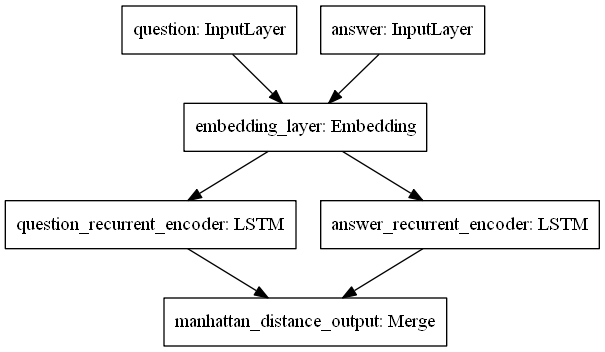
\includegraphics[scale=0.4]{subtask_a_recurrent_model}
\centering
\end{figure}

Sieć została również przeuczona zbiorem trenującym, a następnie jej skuteczność została sprawdzona zbiorem walidującym. Poniżej zamieszczono wykresy przedstawiający przebieg uczenia dla 100 epok (rysunki~\ref{fig:fflossrr} i \ref{fig:ffaccrr}).

\begin{figure}[H]
\centering
\caption{Przebieg uczenia sieci syjamskiej dla 100 epok (strata). \label{fig:fflossrr}}
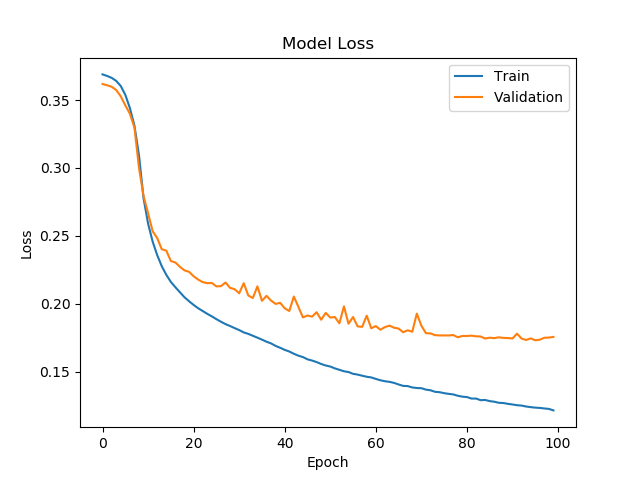
\includegraphics[scale=0.7]{subtask_a_recurrent_loss.png}
\end{figure}


\begin{figure}[H]
\centering
\caption{Przebieg uczenia  sieci syjamskiej  dla 100 epok (trafność). \label{fig:ffaccrr}}
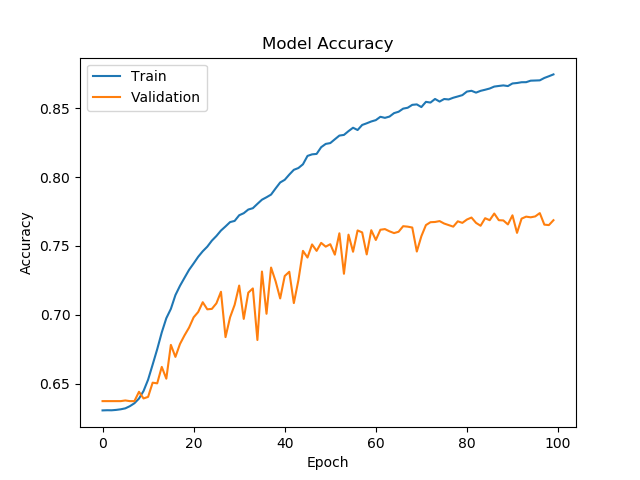
\includegraphics[scale=0.7]{subtask_a_recurrent_acc.png}
\end{figure}


\begin{table}[H]
\caption{Skuteczność sieci syjamskiej na zbiorze uczącym.}
\label{train_set_statistics_score_table}
    \begin{center}
        \begin{tabular}{ |c|c| } 
            \hline
            metryka & wartość\\
            \hline
            Accuracy & 0,883 \\
            \hline
            Precision & 0,877 \\
            \hline
            Recall & 0,796\\ 
            \hline
        \end{tabular}
    \end{center}
\end{table}

\begin{table}[H]
\caption{Skuteczność sieci syjamskiej na zbiorze testowym.}
\label{train_set_statistics_score_table}
    \begin{center}
        \begin{tabular}{ |c|c| } 
            \hline
            metryka & wartość\\
            \hline
            Accuracy & 0,768 \\
            \hline
            Precision & 0,589 \\
            \hline
            Recall & 0,721 \\ 
            \hline
        \end{tabular}
    \end{center}
\end{table}

\subsection{Rozszerzenie zbioru danych}
Jednym ze sposobów zwiększenia skuteczności modeli opartych o uczenie maszynowe jest wytrenowanie ich na większej ilości danych. Niestety nie było możliwości pozyskania nowych przykładów uczących. Problem ten rozwiązano techniką polegającą na sztucznym powiększeniu zbioru danych o nowe przypadki. Na podstawie oryginalnego zbioru został stworzony zbiór rozszerzony, w którym nowe próbki utworzono zamieniając niektóre wyrazy na ich synonimy. 
Dokładną charakterystykę zbioru oryginalnego i rozszerzonego przedstawia tablica~\ref{a_augmented_set_percentage}.

\begin{table}[H]
\caption{Rozkłady ilościowe klas w zbiorze oryginalnym i rozszerzonym.}
\label{a_augmented_set_percentage}
    \begin{center}
        \begin{tabular}{ |c|c|c|c| } 
            \hline
            Zbiór & Liczność zbioru & ,,Good'' & ,,Bad''\\
            \hline
            Oryginalny & 30242 & 36,27\% & 63,04\%\\
            \hline
            Rozszerzony & 124368 & 35.76\% & 64,24\%\\ 
            \hline
        \end{tabular}
    \end{center}
\end{table}

Na zbiorze rozszerzonym został wytrenowany wcześniej przedstawiony model sieci syjamskiej. Wyniki przedstawiają rysunki~\ref{a_siamese_augmented_acc} i \ref{a_siamese_augmented_loss}.

\begin{figure}[H]
\centering
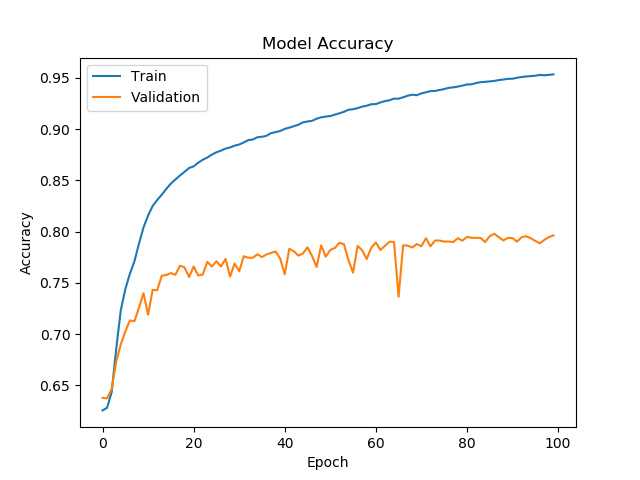
\includegraphics[scale=0.5]{subtask_a_recurrent_augmented_acc}
\caption{Trafność sieci syjamskiej na zbiorze rozszerzonym.}
\label{a_siamese_augmented_acc}
\end{figure}

\begin{figure}[H]
\centering
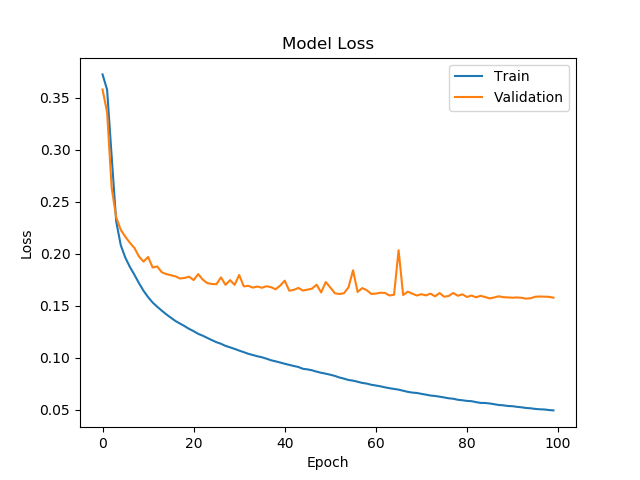
\includegraphics[scale=0.5]{subtask_a_recurrent_augmented_loss}
\caption{Strata sieci syjamskiej na zbiorze rozszerzonym.}
\label{a_siamese_augmented_loss}
\end{figure}


\begin{table}[H]
\caption{Skuteczność sieci syjamskiej na zbiorze rozszerzonym.}
\label{train_set_statistics_score_table_augmented}
    \begin{center}
        \begin{tabular}{ |c|c| } 
            \hline
            metryka & wartość\\
            \hline
            Accuracy & 0.955 \\
            \hline
            Precision & 0.955 \\
            \hline
            Recall & 0.923\\ 
            \hline
        \end{tabular}
    \end{center}
\end{table}

\begin{table}[H]
\caption{Skuteczność sieci syjamskiej na zbiorze testowym.}
\label{train_set_statistics_score_table_augmented}
    \begin{center}
        \begin{tabular}{ |c|c| } 
            \hline
            metryka & wartość\\
            \hline
            Accuracy & 0.796 \\
            \hline
            Precision & 0.633 \\
            \hline
            Recall & 0.764 \\ 
            \hline
        \end{tabular}
    \end{center}
\end{table}

Trafność działania modelu na zbiorze walidującym została zwiększona, osiągnęła ostatecznie wynik około 79\%.

\subsection{Ocena rezultatów}
Analizując wyniki otrzymane po wyuczeniu modelu sieci syjamskiej można stwierdzić że wykorzystanie rozszerzonego zbioru danych podnosi jakość klasyfikacji. Trafność wzrosła z 76.8\% do 79.6\% co stanowi redukcję błędu o 12\%.